\section{Geometry and Motion}
\subsection*{Geometry of a tetrahedron}
\smallskip

A \textbf{face} \{{$^i{\underline{\mathbf{x}}}$,$^j{\underline{\mathbf{x}}}$,$^k{\underline{\mathbf{x}}}$}\} is parametrized by: \\
{$\underline{\mathbf{x}} = \tensor[^i]{b}{} \tensor[^i]{\underline{\mathbf{x}}}{} + \tensor[^j]{b}{} \tensor[^j]{\underline{\mathbf{x}}}{} + \left(1- \tensor[^i]{b}{} - \tensor[^j]{b}{} \right) \tensor[^k]{\underline{\mathbf{x}}}{}$} \\

An \textbf{edge} \{{$^i{\underline{\mathbf{x}}}$, $^j{\underline{\mathbf{x}}}$,}\} is parametrized by: \\
{$\underline{\mathbf{x}} = \tensor*[^i]{b}{} \tensor[^i]{\underline{\mathbf{x}}}{} + \left(1 - \tensor[^i]{b}{} \right) \tensor[^j]{\underline{\mathbf{x}}}{} $}\\

The  \textbf{length of the edge} \{{$^i{\underline{\mathbf{x}}}$,$^j{\underline{\mathbf{x}}}$,}\} is determined by the norm:
{$\left\lVert \tensor[^i]{\underline{\mathbf{x}}}{} - \tensor[^j]{\underline{\mathbf{x}}}{} \right\rVert $}

The area of the \textbf{face} \{{$^i{\underline{\mathbf{x}}}$,$^j{\underline{\mathbf{x}}}$,$^k{\underline{\mathbf{x}}}$}\} is determined by the norm of the cross product of two edges: \\
{$\frac{1}{2} \left \| \left( \tensor[^i]{\underline{\mathbf{x}}}{} - \tensor[^k]{\underline{\mathbf{x}}}{} \right) \wedge \left( \tensor[^j]{\underline{\mathbf{x}}}{} - \tensor[^k]{\underline{\mathbf{x}}}{}\right)\right\|$}

The \textbf{volume} of the tetrahedron \{{$^1{\underline{\mathbf{x}}}$,$^2{\underline{\mathbf{x}}}$,$^3{\underline{\mathbf{x}}}$,$^4{\underline{\mathbf{x}}}$}\} is given by the mixed product: \\
{$ V = \frac{1}{6} \left(\tensor[^3]{\underline{\mathbf{x}}}{} - \tensor[^4]{\underline{\mathbf{x}}}{} \right) \cdot \left [ \left(\tensor[^1]{\underline{\mathbf{x}}}{} - \tensor[^4]{\underline{\mathbf{x}}}{} \right) \wedge \left(\tensor[^2]{\underline{\mathbf{x}}}{} - \tensor[^4]{\underline{\mathbf{x}}}{} \right) \right ]$} \\


\subsection*{Translations and Rotations}
\smallskip
The description based on an original configuration where each particle is followed up in time is named \textbf{Lagrangean}.\\

\begin{center}
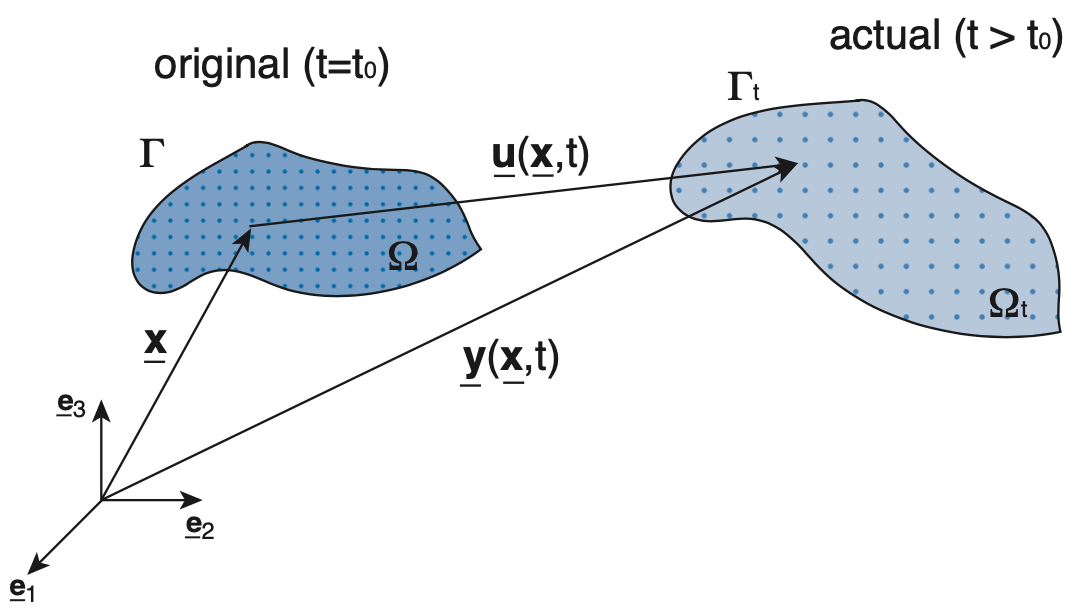
\includegraphics[width=0.5\linewidth]{img/Configurations} \\
\end{center}

\textbf{Final position:} {$\tensor[^i]{\underline{\mathbf{y}}}{} = {\underline{\underline{R}}} \tensor[^i]{\underline{\mathbf{x}}}{} + \underline{\mathbf{b}} \qquad i = 1,4 $} \\
With $ {\underline{\underline{R}}} = \left[\begin{array}{ccc}cos(\theta) & -sin(\theta) & 0 \\sin(\theta) & cos(\theta) & 0 \\0 & 0 & 1\end{array}\right]$ along axis $ \tensor[^3]{\underline{\mathbf{e}}}{}$ \ and $\quad \underline{\mathbf{b}} = \left[\begin{array}{c}0 \\0 \\n\end{array}\right]$ \\

Rotation matrix is \textbf{orthogonal}: $ {\underline{\underline{R^T}}} \underline{\underline{R}} = \underline{\underline{I}}$ \\

\textbf{Displacements:} {$ \tensor[^i]{\underline{\mathbf{u}}}{}(\underline{\mathbf{x}}, t) = \tensor[^i]{\underline{\mathbf{y}}}{}(\underline{\mathbf{x}}, t) - \tensor[^i]{\underline{\mathbf{x}}}{} \qquad i = 1,4 $} \\
\textbf{Velocities:} $\underline{\dot{\mathbf{y}}}(\underline{\mathbf{x}}, t) \equiv \diffp{\underline{\mathbf{y}}}{t}(\underline{\mathbf{x}}, t)$ \\
\textbf{Accelerations:} $\underline{\ddot{\mathbf{y}}}(\underline{\mathbf{x}}, t) \equiv \diffp[2]{\underline{\mathbf{y}}}{t}(\underline{\mathbf{x}}, t)$ \\


Motion is \textbf{bijective}: each beginning point has only $1$ ending point. This implies the existence of an inverse motion: $ \underline{y}^{-1} (\underline{y} (\underline{x},t),t) = \underline{x}$ \\

Rigid Body motion conserves volume: $ \Vert  \underline{y} - \underline{\tilde{y}} \Vert = \Vert  \underline{x} - \underline{\tilde{x}} \Vert$, but orientation is lost!

\lstinputlisting[style=Matlab-editor,basicstyle=\color{black}\ttfamily\normalsize, firstline=3, lastline=5]{CheatSheet.m}

\textbf{Gradient of displacement:} \\
$\underline{\underline{H}}(\underline{x},t) = \nabla_{\underline{x}} \underline{u} (\underline{x},t) = \left[\begin{smallmatrix} \frac{\delta u_1}{\delta x_1} & \frac{\delta u_1}{\delta x_2} & \frac{\delta u_1}{\delta x_3} \\ \frac{\delta u_2}{\delta x_1} & \frac{\delta u_2}{\delta x_2} & \frac{\delta u_2}{\delta x_3} \\ \frac{\delta u_3}{\delta x_1} & \frac{\delta u_3}{\delta x_2} & \frac{\delta u_3}{\delta x_3} \end{smallmatrix}\right] $\\
\textbf{Gradient of motion:}  $ \underline{\underline{F}} \rightarrow \underline{\underline{H}} = \underline{\underline{F}} - \underline{\underline{I}} $


$d \underline{u} = \underline{\underline{H}} d \underline{x} = \nabla_{\underline{x}} \underline{u} d \underline{x}$ \\
$= \underbrace{\frac{1}{2} (\underline{\underline{H}} + \underline{\underline{H}}^T)}_{\text{symmetric}} +  \underbrace{\frac{1}{2} (\underline{\underline{H}} - \underline{\underline{H}}^T)}_{\text{anti-symmetric}} $ \\
$= (\underline{\underline{\epsilon}} + \underline{\underline{A}}) d \underline{x} $


\subsection*{Coordinate System}
\smallskip

\textbf{Reference frame:} \begin{enumerate}
\item N points ($ N \geqslant 4 $ in 3D)
\item Non coplanar
\item Immobile
\item In fact, a \textbf{rigid body}
\end{enumerate}

\textbf{Orthogonal transformation $Q_{ij}$:} \\
A square matrix $\mathbf{Q}$ is \textit{orthogonal} if $\mathbf{Q}^{-1} = \mathbf{Q}^T$
\begin{itemize}
\item if $ \det{Q_{ij}} = +1$: orientation conserved;
\item if $ \det{Q_{ij}} = -1$: orientation inversed.
\end{itemize}

\textbf{Change into new CS:}
\begin{itemize}
\item Scalars $\alpha ' = \alpha$ $\rightarrow$ invariant
\item Vectors $v_i = Q_{ij}v_j$
\item Tensors of Order 2 $T'_{ij} = Q_{ik}Q_{jl}T_{kl}$
\end{itemize}

A \textbf{tensor of order n} is an object that needs n applications of the transformation $Q_{ij}$ to characterise the change of its components:
$C_{ij...n} '= Q_{ik} Q_{jl} ... Q_{nm} C_{kl...m}$ \\

\textbf{Isomorphism between $R^3$ × $R^3$ and $R^9$:} \\
$ \left[\begin{array}{ccc}T_{11} & T_{12} & T_{13} \\T_{21} & T_{22} & T_{23} \\T_{31} & T_{32} & T_{33}\end{array}\right] \leftrightarrow \left[\begin{array}{c}T_{11} \\T_{12} \\T_{13} \\T_{21} \\T_{22} \\T_{23} \\T_{31} \\T_{32} \\T_{33}\end{array}\right] $